\chapter{Resultados}

\section{Separação de padrões}


Alguns resultados iniciais a partir do protocolo descrito na Seção~\ref{sec:separacao_padroes} já foram obtidos e serão discutidos
nesta seção.

A Figura~\ref{fig:avg_activity} apresenta a ativação média das populações de GCs para o modelo de controle (sem neurogênese) e
para os modelos com neurogênese em diferentes níveis de conectividade das iGCs com o CE. No modelo de controle, onde todas as GCs
são maduras, a ativação média da população foi de 12.46\%, um nível que reflete aproximadamente a ativação esparsa característica
do GD.

A introdução de iGCs no circuito altera significativamente essa dinâmica. Conforme a conectividade das iGCs aumenta, a sua taxa de
ativação cresce acentuadamente, o que é consistente com sua maior excitabilidade intrínseca. No cenário de 100\% de conectividade,
praticamente toda a população de iGCs se torna ativa em resposta a um padrão de entrada. Esse aumento na atividade das iGCs eleva
a ativação geral da população de GCs.

Em contrapartida, observa-se uma diminuição progressiva na atividade das GCs maduras (mGCs) à medida que a conectividade das iGCs
aumenta. Este resultado sugere a existência de um mecanismo de competição inibitória, onde as iGCs, ao serem fortemente ativadas,
acabam por suprimir indiretamente a atividade das mGCs através dos interneurônios compartilhados.

Contudo, a supressão observada nas mGCs não é tão acentuada quanto a reportada em outros modelos~\cite{kimEffect2024a}, o que pode
indicar que a força da inibição no modelo atual seja insuficiente. Uma hipótese para essa discrepância é a ausência de uma via
inibitória direta das iGCs para as mGCs, um mecanismo descrito por~\citeonline{lunaAdultborn2019} que não foi implementado. A
inclusão dessa conexão direta é uma via promissora para futuras investigações, podendo conferir maior realismo biológico ao
modelo.

\begin{figure}[H]
    \centering
    \caption{Ativação média da população (\%) por modelo.}
    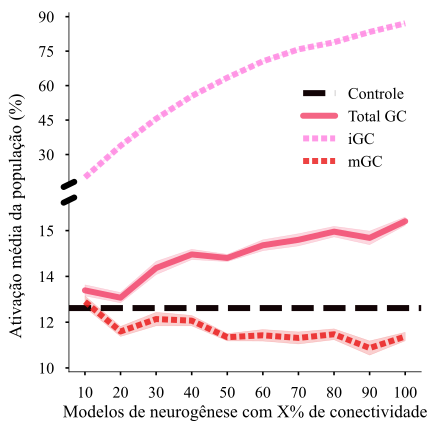
\includegraphics[width=0.7\textwidth]{figuras/plots/avg_activity}
    \label{fig:avg_activity}
\end{figure}

\begin{figure}
    \centering
    \caption{Grau de separação de padrões ($\mathcal{S}_D$) por modelo.}
    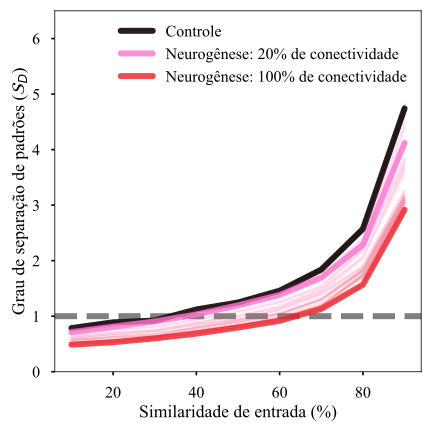
\includegraphics[width=0.7\textwidth]{figuras/plots/pattern_separation}
    \label{fig:pattern_separation}
\end{figure}

\begin{figure}
    \centering
    \caption{Grau de separação de padrões ($\mathcal{S}_D$) médio por modelo.}
    \includegraphics[width=0.7\textwidth]{figuras/plots/avg_pattern_separation}
    \label{fig:avg_pattern_separation}
\end{figure}


\section{Resultados esperados}

Espera-se que a presença de iGCs prejudique o completamento de padrões no CA3, devido a uma maior ativação de assembleias
neuronais não relacionadas ao padrão de entrada, um efeito consistente com resultados experimentais que sugerem uma ativação
promíscua de assembleias por parte das iGCs devido à sua alta excitabilidade~\cite{koSystems2025}. Adicionalmente, na simulação da
maturação temporal, espera-se que as iGCs passem a codificar os padrões no tempo, integrando informações que foram apresentadas
enquanto eram jovens, corroborando seu papel como integradoras temporais, como proposto por~\cite{aimoneComputational2009}.
Teoriza-se, portanto, que as mGCs teriam um papel predominante na separação de padrões específicos e distintos, enquanto as iGCs,
ao longo de sua maturação, se especializariam na separação de padrões próximos no tempo, ou seja, aqueles que codificaram durante
sua fase imatura.
